\documentclass{article}
\usepackage{arxiv}
\usepackage[utf8]{inputenc}
\usepackage[T1]{fontenc}
\usepackage{hyperref}
\usepackage{url}
\usepackage{booktabs}
\usepackage{amsfonts}
\usepackage{amsmath}
\usepackage{nicefrac}
\usepackage{microtype}
\usepackage{cleveref}
\usepackage{graphicx}
\usepackage{natbib}
\usepackage{array}
\usepackage{multirow}
\usepackage{float}
\usepackage{CJKutf8}

\graphicspath{{figs/}{.}}

\title{SILP: A Semantic Interlingua Layer Protocol for Cross-Model Agent Communication}

\newif\ifuniqueAffiliation
\uniqueAffiliationtrue

\ifuniqueAffiliation
\author{
  \href{https://orcid.org/0009-0007-9231-8698}{
\includegraphics[scale=0.06]{orcid.pdf}\hspace{1mm}Juwan Hwang (\begin{CJK}{UTF8}{gbsn}黄治文\end{CJK})} \\
  Shanghai Maritime University \\
  Shanghai, China \\
  \texttt{huangzhiwen@stu.shmtu.edu.cn} \\
}
\fi

\renewcommand{\shorttitle}{SILP: Semantic Interlingua Layer Protocol}

\hypersetup{
  pdftitle={SILP: A Semantic Interlingua Layer Protocol for Cross-Model Agent Communication},
  pdfsubject={cs.CL, cs.AI, cs.MA},
  pdfauthor={Juwan Hwang},
  pdfkeywords={LLM, agent communication, protocol, interlingua, prompt compression},
}

\begin{document}
\maketitle

\begin{abstract}
Large language models (LLMs) increasingly communicate with one another through text-based agent protocols such as MCP and A2A, yet the encoding of semantic payloads in these protocols remains unspecified. We introduce SILP (Semantic Interlingua Layer Protocol), a black-box, text-interface payload codec that compiles a coarse-grained action-slot intermediate representation (IR) into multiple pluggable surface frontends---code-like function-call syntax, pure JSON, natural language, and ML-compressed text---each designed to exploit the shared training priors of contemporary LLMs. We empirically test the central hypothesis that \emph{shared syntactic priors} (code-format familiarity from pretraining) contribute more to cross-model comprehension than \emph{shared vocabulary priors} (word-level semantics). Across four main phases plus a smoke-test subphase spanning 5 frontends, 6 tokenizers, 5 API-reported model endpoints, and 27 semantically diverse test cases (3,159 total model invocations; counting methodology defined in \S3.7), we find: (1) the code frontend achieves the highest average pass rate (85.9\%, statistically tied with JSON at 84.4\% and natural language at 83.0\%, McNemar p > 0.59) with the lowest cross-tokenizer variance (range 2--10 tokens); (2) ablation reveals that removing vocabulary semantics collapses pass rates to 1.2\% (skeleton condition), while word-order shuffling reduces them to 55.6\% (shuffled condition), indicating \emph{both} perturbations caused significant performance drops but, contrary to the original hypothesis, semantic-vocabulary removal caused a larger performance drop than word-order disruption (85.2 vs.~30.8 percentage-point performance drops under two distinct perturbations, a 2.8$\times$ descriptive ratio); (3) under the tested LLMLingua-2 configuration (rate=0.5), the code frontend achieves a 60.0-percentage-point higher pass rate; and (4) in multi-turn sessions of up to 15 rounds, we detect no statistically significant evidence of error propagation or pass-rate degradation (Fisher exact test, p $\geq$ 0.10; Benjamini--Hochberg FDR corrected), although the experiment is underpowered for small deep-context effects. We release the implemented codec, benchmark harness, protocol specification, and all raw data as open-source at https://github.com/Juwan-Hwang/polyglotir.
\end{abstract}

\section{Introduction}\label{introduction}



The rise of agentic AI systems has created a new communication paradigm: large language models (LLMs) conversing not with humans, but with other LLMs through structured text protocols. Frameworks such as the Model Context Protocol (MCP) and Agent-to-Agent (A2A) protocol define transport envelopes and capability discovery, but leave a critical gap: \emph{how should the semantic payload itself be encoded?} Current practice defaults to uncompressed natural language, which is token-inefficient, tokenizer-dependent, and semantically ambiguous---particularly for negation logic, multi-step action chains, and conditional branching.



This paper introduces SILP (Semantic Interlingua Layer Protocol), a five-layer protocol stack that addresses this gap. SILP defines a coarse-grained action-slot intermediate representation (IR) as the canonical semantic layer, compiles it into multiple pluggable ``frontends'' (surface encodings), and provides a negotiation layer for dynamic frontend selection. The design is grounded in a central testable question: do \textbf{shared syntactic priors} (code-format familiarity from pretraining) or \textbf{shared vocabulary priors} (word-level semantics) contribute more to cross-model comprehension? The intuitive prediction is that syntax dominates---modern LLMs have seen millions of code snippets in training, so structuring agent-to-agent payloads as code-like syntax should yield better comprehension than natural language or ML-based compression, without fine-tuning or model-internal access. Our ablation results (\S4.5) contradict this prediction: removing semantic vocabulary caused a 2.8$\times$ larger performance drop than shuffling syntactic order, though both perturbations produced statistically significant effects. This reversal is a primary finding of the paper, not a limitation.



We evaluate SILP through four main phases and an intermediate smoke-test subphase:



\begin{itemize}



\item

  \textbf{Phase 0}: Cross-tokenizer census verifying that SILP's vocabulary and syntax tokens are single-token, low-variance, and UNK-free across six production tokenizers (\S4.1).

\item

  \textbf{Phase 0.5}: Smoke test validating end-to-end pipeline integrity with compile.lock physical freezing (\S4.2).

\item

  \textbf{Phase 1}: Infrastructure validation including collision testing and round-trip losslessness (\S4.3).

\item

  \textbf{Phase 2}: Generalizability benchmark matrix---5 frontends $\times$ 5 models $\times$ 27 cases = 675 runs---measuring relative pass rates, cross-model case-level agreement, and the compression--accuracy tradeoff (\S4.4).

\item

  \textbf{Phase 3}: Three sub-experiments: (a) ablation isolating syntax vs.~vocabulary contributions, (b) entropy analysis relating information density to pass rates, and (c) heartbeat experiment testing error propagation across 2,160 multi-turn runs (\S4.5--4.7).

\end{itemize}



\textbf{Contributions.} This paper makes three contributions:



\begin{enumerate}


\item

  \textbf{Protocol architecture}: SILP---a five-layer, plug-in-based payload codec with a semantically auditable IR, multiple surface frontends, and a negotiation layer---designed as a payload layer for MCP/A2A, not a compression tool.

\item

  \textbf{Empirical evidence on prior decomposition}: Through ablation, we falsify the original hypothesis's directional prediction---removing semantic vocabulary caused a 2.8$\times$ larger performance drop than shuffling syntactic order (85.2 vs.~30.8 percentage points), though both perturbations produced statistically significant effects. This reframes the central question: the tested models were more sensitive to semantic-vocabulary removal than to word-order disruption.

\item

  \textbf{Benchmark and data}: The first ``frontend $\times$ API-reported model endpoint'' generalizability matrix (5$\times$5$\times$27 = 675 runs) with an LLM-judge evaluation protocol (with rule-based fallback and audit signal), compression--accuracy tradeoff curves, and multi-turn error propagation analysis---all released as open-source with raw data.

\end{enumerate}



\section{Related Work}\label{related-work}



\textbf{Prompt compression.} LLMLingua \citep{jiang2023llmlingua} and LLMLingua-2 \citep{pan2024llmlingua2} use perplexity-based and token-level ML compression to reduce prompt length. These methods optimize for token reduction but may sacrifice semantic precision---our Phase 2 results show that under the tested configuration (rate=0.5), LLMLingua-2 reduces average character length by 45.8\% but attains only a 25.9\% pass rate, whereas the code frontend is 3.2\% shorter than natural language by character count and attains 85.9\%. SILP differs fundamentally: it is a \emph{protocol layer} (lossless, auditable, negotiable) rather than a \emph{compression tool} (lossy, opaque, one-shot).



\textbf{Learned message representation.} A concurrent line of work asks a complementary question: rather than testing \emph{why} certain representations succeed, OPTiMACS \citep{gupta2026learning} frames message-format selection for agentic communication as a reinforcement-learning problem, learning task-conditional optimal formats (JSON, propositions, code, etc.) via an Expanding Markov Decision Process. This approach can adaptively select formats per-task but requires online policy learning and does not isolate \emph{which} component of a representation---its vocabulary or its syntax---drives comprehension. SILP instead operates zero-shot and provides a mechanistic decomposition (\S4.5) of this question, which is orthogonal to OPTiMACS's format-selection objective; the two approaches could in principle be composed.



\textbf{Emergent communication.} The emergent communication literature \citep{havrylov2017emergence, lazaridou2017multiagent} studies how agents develop shared signaling systems from scratch, typically through reinforcement learning. SILP differs by leveraging \emph{pre-existing} shared priors from pretraining---no learning is needed. Agents use code-like syntax they have already seen millions of times in training data, making communication zero-shot and immediately interpretable.



\textbf{Structured prompting.} Methods like StructGPT \citep{jiang2023structgpt} use structured prompts (JSON, SQL-like syntax) to improve LLM reasoning. These approaches are task-specific and do not define a generalizable inter-agent payload protocol. SILP provides a formal protocol stack with compile/decode round-trip guarantees, negotiation, and multi-frontend support.



\textbf{Agent communication protocols.} MCP \citep{anthropic2024mcp} and A2A \citep{google2024a2a} define transport-level and capability-discovery semantics but do not standardize payload encoding. SILP is designed as a payload-layer option within these frameworks---it sits inside MCP's \texttt{params} or A2A's \texttt{task/message/artifact} fields without replacing their lifecycle management.



\textbf{Agent network architectures.} At a more macro architectural level, \citet{zhang2026agentnetwork} propose a vision for open multi-agent connectivity centered on a ``dual narrow-waist'' design, in which the Task Semantic Intermediate Representation (TSIR) serves as a semantic waist for circulating task intent---conceptually analogous to SILP's Layer 1 IR. The authors explicitly note that theirs is a position paper: ``we do not present a complete protocol specification or a performance evaluation.'' SILP complements this direction by providing a concrete, implemented, and empirically validated instantiation of a semantic-waist-like layer, including a compile/decode-guaranteed codec, a negotiation mechanism, and quantitative evidence (via ablation) on what drives cross-model comprehension at the payload level.



\textbf{Interlingua in NLP.} The concept of an interlingua---an intermediate representation that mediates between input and output languages---has a long history in machine translation \citep{hutchins1995mt}. SILP adapts this concept to the LLM-agent domain: the IR is the interlingua, and frontends are the ``target languages'' compiled from it. Unlike AMR \citep{banarescu2013amr}, which is a graph-semantic representation, SILP's IR is a coarse-grained action-slot structure optimized for text-interface compilation rather than graph traversal.



\section{Methods}\label{methods}



\subsection{SILP Protocol Architecture}\label{silp-protocol-architecture}



SILP is a five-layer protocol stack:



\textbf{Layer 1 --- Application Layer (Semantic IR).} The canonical intermediate representation is a JSON-serialized action-slot structure with four top-level fields: \texttt{intent} (the primary action, e.g., \texttt{!CANCEL}), \texttt{entities} (argument slots), \texttt{constraints} (conditions), and \texttt{alternatives} (else-branch actions). A \texttt{meta} object carries protocol-level metadata: \texttt{req\_id} (8 hex chars by default; 4 only in scope-limited sessions), \texttt{session\_id} (for stateful mode), \texttt{out} (output format hint), and \texttt{next\_agent} (routing). The IR is defined as a Pydantic v2 model with strict validation: the root is \texttt{extra="forbid"} (no unknown fields), while sub-models allow extensibility. Action codes follow the format \texttt{!} + \texttt{UPPERCASE\_VERB} (e.g., \texttt{!CANCEL}, \texttt{!START}) and are validated by regex.



\textbf{Layer 2 --- Surface Layer (Pluggable Frontends).} Five frontends compile IR $\to$ surface string:



\begin{table}[ht]
\centering
\small
\caption{The five surface frontends. \texttt{code} and \texttt{json} are lossless codecs (decode(compile(ir)) $\equiv$ ir). \texttt{natural}, \texttt{nl\_json}, and \texttt{llmlingua2} are control baselines that cannot be decoded.}
\begin{tabular}{lll}
\toprule
Frontend & Description & Round-trip? \\
\midrule
\texttt{code} & Function-call syntax: \texttt{if\ !rain(t+1):\ start(hike)\ else\ start(cards@indoor)} & Yes (lossless) \\
\texttt{json} & Flat JSON slots: \texttt{\{"intent":"!CANCEL","act":"flight",...\}} & Yes (lossless) \\
\texttt{natural} & Unstructured prose: ``If not rain at t+1, start hike otherwise start cards at indoor.'' & No (control) \\
\texttt{nl\_json} & Natural language wrapped in JSON: \texttt{\{"task\_description":"..."\}} & No (control) \\
\texttt{llmlingua2} & LLMLingua-2 compressed natural language (rate=0.5) & No (lossy) \\
\bottomrule
\end{tabular}
\end{table}


The \texttt{code} frontend maps IR action codes to lowercase function calls (\texttt{!CANCEL} $\to$ \texttt{cancel()}), compiles constraints as boolean conditions (\texttt{if\ loc(me,Beijing,t+1am):}), entities as positional or keyword arguments, and alternatives as \texttt{else:} branches. The \texttt{json} frontend renders the IR as a flat JSON object with only semantic slots---no code syntax---to isolate ``format contribution'' from ``code vocabulary prior.'' The \texttt{nl\_json} frontend wraps the \emph{exact same prose} as \texttt{natural} inside a JSON \texttt{task\_description} field, isolating the JSON-container effect from content differences. The \texttt{llmlingua2} frontend compresses the \texttt{natural} rendering using Microsoft's LLMLingua-2 (XLM-RoBERTa-large, rate=0.5), serving as the compression-tool baseline.



\textbf{Layer 3 --- Meta-protocol Layer.} Handles dynamic frontend negotiation via a \texttt{//ping} probe, session management (2-char session IDs, heartbeat renewal every N turns), error codes (invalid\_syntax, unsupported\_version, etc.), and degradation chains (code $\to$ math $\to$ JSON $\to$ natural language).



\textbf{Layer 4 --- Optimization Layer.} A multi-objective fitness function: \texttt{Fitness\ =\ $\alpha$$\cdot$task\_success\ +\ $\alpha$\textquotesingle{}$\cdot$cross\_model\_fidelity\ +\ $\beta$$\cdot$compression\ -\ $\gamma$$\cdot$human\_unreadability\ -\ $\delta$$\cdot$PPL\ -\ $\varepsilon$$\cdot$tokenizer\_variance\ -\ $\zeta$$\cdot$cross\_model\_ambiguity}, constrained by $\alpha$ + $\alpha$' $\geq$ 0.6 and a hard fidelity floor.



\textbf{Layer 5 --- Migration Layer.} Proposed migration screening layer, intended to test ranking preservation: if small models and API-reported endpoints rank frontends similarly (high Spearman $\rho$), small models could serve as proxies for frontend evaluation. Not yet validated.



\subsection{Test Case Design}\label{test-case-design}



We designed 27 IR test cases across 9 semantic categories, each with 3 difficulty variants (baseline, complex, adversarial):



\begin{table}[ht]
\centering
\footnotesize
\caption{The 9 semantic categories (27 cases total = 9 $\times$ 3 variants). Cases span negation logic, conditional branching, multi-step chains, nested constraints, and tool invocation---representing the structural diversity of agent-to-agent communication.}
\begin{tabular}{l>{\raggedright\arraybackslash}p{2cm}>{\raggedright\arraybackslash}p{9cm}>{\raggedright\arraybackslash}p{2cm}}
\toprule
\# & Category & Example (code frontend) & Key Challenge \\
\midrule
1 & Multi-constraint logic & \texttt{if\ loc(me,Beijing,t+1am):\ cancel(flight,t+1pm);\ email(zhangsan)} & Simultaneous constraints + secondary action \\
2 & \textbf{Negation logic} & \texttt{if\ !rain(t+1):\ start(hike)\ else\ start(cards@indoor)} & Correct negation handling (critical for hypothesis) \\
3 & Detail preservation & \texttt{translate(src=fr\_rev\_bold,\ tgt=shakespeare\_en,\ style=archaic\_heavy)} & Four parameters, compound values \\
4 & Tool-call branching & \texttt{if\ weather>rain\ then\ switch\_tool(indoor\_activity)} & Operator conditions, tool switching \\
5 & Nested constraints & \texttt{if\ budget<=500\ and\ rating>=4.0:\ book(hotel,downtown,t+5)} & Multiple inequality constraints \\
6 & Parallel actions & \texttt{fetch(data)\ ->\ process\ ->\ email(result)\ with\ timeout} & Sequencing, timeout constraint \\
7 & Conditional branching & \texttt{if\ urgency>high:\ route(ticket)\ else\ escalate(manager)} & If-else routing logic \\
8 & Tool invocation & \texttt{search(restaurants,italian,Beijing,open\_now)} if rating\textgreater=4.5 & Multi-argument search + constraint \\
9 & Multi-turn state & \texttt{update(order\_42,\ address,\ 5\_Tianfu\_Ave)} & Stateful parameter tracking \\
\bottomrule
\end{tabular}
\end{table}


\subsection{Models}\label{models}



Five API-reported model endpoints accessed through an OpenAI-compatible proxy:



\begin{table}[ht]
\centering
\small
\begin{tabular}{lll}
\toprule
Model & Family & Access \\
\midrule
DeepSeek-v3.2 & DeepSeek & API (proxy) \\
GLM-5.2 & Zhipu/GLM & API (proxy) \\
Kimi-K2.6 & Moonshot/Kimi & API (proxy) \\
LongCat-2.0 & Meituan/LongCat & API (proxy) \\
MiniMax-M2.7 & MiniMax & API (proxy) \\
\bottomrule
\end{tabular}
\end{table}


All models were accessed via the same OpenAI-compatible endpoint with greedy decoding (temperature=0, max\_new\_tokens=256). Three local small models (SmolLM-360M, Qwen2.5-0.5B, TinyLlama-1.1B) were used for CPU-level pre-filtering but are not included in the main results.



\subsection{Evaluation: Primary LLM Judge with Rule-Based Fallback}\label{evaluation-primary-llm-judge-with-rule-based-fallback}



We use a \textbf{primary LLM judge with a rule-based fallback} to evaluate whether a model's response correctly captures the IR's semantic intent:



\begin{enumerate}


\item

  \textbf{LLM Judge (primary)}: A separate model (GLM-5.2) receives the original IR, the encoded instruction shown to the model, and the model's response. It evaluates six criteria: main action, all entities/arguments, all constraints/conditions, negation logic (reversed negation = automatic fail), alternative/else-branch, and ordering. The judge prompt is \emph{fixed}---no per-case tuning.

\item

  \textbf{Rule Judge (secondary, recorded)}: A lightweight heuristic checks for key entities, verbs, and negation markers in the response, with bilingual (English--Chinese) synonym tables. Its false-negative rate in cross-lingual scenarios is itself a measurable metric.

\end{enumerate}



The LLM judge verdict is primary for pass-rate calculation. If the LLM judge errors (proxy down), the rule judge verdict is used as fallback with a flag. All judgments are logged for full audit.



\subsection{Tokenizer Census}\label{tokenizer-census}



Six production tokenizers were surveyed: gpt-4o (tiktoken), gpt-3.5 (tiktoken), llama-2 (SentencePiece), qwen2.5 (SentencePiece), claude (custom), and gemini (SentencePiece). For each of the 15 whitelisted verbs, 12 structural tokens (\texttt{if}, \texttt{else}, \texttt{and}, \texttt{not}, \texttt{(}, \texttt{)}, \texttt{,}, \texttt{;}, \texttt{:}, \texttt{!}, \texttt{@}, \texttt{->}), and the 9 baseline test cases compiled under each frontend, we measured: single-token status, token count, UNK presence, and cross-tokenizer variance.



\subsection{Statistical Methods}\label{statistical-methods}



\begin{itemize}



\item

  \textbf{Pass rates}: Binary pass/fail per run, aggregated as proportions.

\item

  \textbf{Cross-model case-level agreement}: Spearman's $\rho$ between each pair of models' per-case-per-frontend binary pass/fail outcomes (n=135 data points per pair = 27 cases $\times$ 5 frontends, threshold=30).

\item

  \textbf{Ablation significance}: McNemar's test (paired, since same cases under different conditions) with Bonferroni correction within the ablation family. Separately, for a project-wide multiplicity analysis, Benjamini--Hochberg FDR was applied to the \emph{unadjusted} p-values from all 35 tests. We do not apply BH to already-Bonferroni-adjusted p-values.

\item

  \textbf{Error propagation}: Fisher's exact test (two-sided), odds ratios with 95\% Woolf confidence intervals.

\item

  \textbf{Trend analysis}: Spearman's $\rho$ between pass rate/latency and context depth.

\item

  \textbf{Multiple comparison correction}: Benjamini--Hochberg FDR across all 35 hypothesis tests reported in this paper (see Appendix B for the complete itemized list).

\end{itemize}



\subsection{Data Integrity Protocol}\label{data-integrity-protocol}



Three strict rules were enforced throughout:



\begin{enumerate}


\item

  \textbf{No error results recorded}: Infrastructure errors (timeout, 5xx, 401, empty response) trigger automatic retry with exponential backoff ($\geq$10 outer rounds). Semantic failures (model answered but wrong) are \emph{never} retried.

\item

  \textbf{No data overwriting}: Resumed runs skip completed (model, N, seed, turn) tuples via incremental append. The original 810-run heartbeat dataset was backed up before expansion.

\item

  \textbf{Compile.lock}: Phase 0.5 introduced a physical freeze---\texttt{silpc} compile generates \texttt{.silp/compile.lock} mapping IR hash $\to$ \{frontend output, timestamp, git\_commit\}, making ``first-pass'' results tamper-evident.

\end{enumerate}



\textbf{Invocation counting methodology.} ``Model invocations'' throughout this paper refers exclusively to \emph{model-under-test} calls---i.e., each unique (model, frontend, case, condition, seed, N, turn) tuple submitted to one of the five API-reported model endpoints for a single generate-and-judge cycle. LLM judge calls (GLM-5.2 evaluating a response) and infrastructure retries (duplicate API calls caused by transient errors) are \emph{not} counted. The per-phase breakdown is: Phase 0.5 = 81 (3 models $\times$ 3 frontends $\times$ 9 cases), Phase 2 = 675 (5 frontends $\times$ 5 models $\times$ 27 cases), Phase 3 ablation = 243 (3 conditions $\times$ 3 models $\times$ 27 cases), Phase 3 heartbeat = 2,160 (3 models $\times$ 8 seeds $\times$ 6 N-values $\times$ 15 turns). \textbf{Total = 3,159.} Phase 0 (tokenizer census) and Phase 1 (collision test, round-trip) involve no model API calls and are excluded. An additional 35 calls were made for a noise-robustness pilot (\S4.6) but that experiment was discontinued and is not counted.



\section{Results}\label{results}



\subsection{Phase 0: Cross-Tokenizer Census}\label{phase-0-cross-tokenizer-census}



\subsubsection{Verb Single-Token Verification}\label{verb-single-token-verification}



All 15 whitelisted verbs were surveyed for single-token status across 6 tokenizers. Of the 15 verbs, 13 are single-token on all 6 tokenizers (cancel, start, email, fetch, process, translate, book, route, search, update, suggest, notify, switch). Two verbs exhibit tokenizer-dependent splitting: \texttt{switch\_tool} (2--3 tokens, never single) and \texttt{escalate} (2--3 tokens, never single). No verb produced a UNK token on any tokenizer (Table: see \texttt{tokenizer\_census\_verbs.csv}).



The 12 structural tokens (\texttt{if}, \texttt{else}, \texttt{and}, \texttt{not}, \texttt{(}, \texttt{)}, \texttt{,}, \texttt{;}, \texttt{:}, \texttt{!}, \texttt{@}, \texttt{->}) are all single-token on all 6 tokenizers with zero UNK occurrences, confirming that the code frontend's syntax vocabulary is universally well-tokenized.



\subsubsection{Cross-Tokenizer Token Variance}\label{cross-tokenizer-token-variance}



For each of the 9 baseline test cases compiled under each frontend, we measured the token count across 6 tokenizers. Figure~\ref{fig:fig3} shows the variance (range = max - min tokens across tokenizers):



\begin{itemize}



\item

  \textbf{Code frontend}: minimum variance (range 2--10 tokens across cases, mean range 5.89). The code frontend's compact function-call syntax produces consistently short encodings across tokenizers.

\item

  \textbf{JSON frontend}: maximum variance (range 7--16, mean range 11.22). The verbose key-value structure amplifies tokenizer differences.

\item

  \textbf{LLMLingua2}: low variance (range 0--7, mean range 3.00) due to aggressive compression, but at the cost of semantic fidelity (see \S4.4).

\item

  \textbf{Natural}: moderate variance (range 2--8, mean range 4.22).

\item

  \textbf{NL+JSON}: moderate variance (range 2--8, mean range 4.89).

\end{itemize}



\begin{figure}[ht]
\centering

\includegraphics[width=0.9\textwidth]{fig3_token_variance}
\caption{Cross-tokenizer token count variance by frontend. Each bar represents the range (max - min) of token counts across 6 tokenizers for a given case--frontend combination. The code frontend exhibits the lowest variance, indicating the most tokenizer-independent encoding.}
\label{fig:fig3}
\end{figure}



The low variance of the code frontend is a direct consequence of its design: function-call syntax (\texttt{cancel(flight)}) uses short, universally-tokenized tokens, while JSON's verbose key names (\texttt{"intent":"!CANCEL","act":"flight"}) introduce tokenizer-dependent splitting.



\subsubsection{Zero-Width and Homoglyph Probes}\label{zero-width-and-homoglyph-probes}



We injected 4 types of zero-width characters (ZWSP, ZWNJ, ZWJ, BOM) into 5 key tokens (cancel, start, translate, if, else) and 1 homoglyph substitution (Latin $\to$ Cyrillic) into 2 tokens (cancel, start), across 6 tokenizers. All 144 probes were detected (survived=True), with token counts increasing by 2--4. This indicates that all tested perturbations altered tokenization and none mapped identically to the unperturbed token sequence under the evaluated tokenizers. However, this does not constitute a complete security guarantee---visual invisibility, preprocessing normalization, and downstream parser behavior are separate concerns not tested here.



\subsection{Phase 0.5: Smoke Test}\label{phase-0.5-smoke-test}



The smoke test validated end-to-end pipeline integrity: 3 models (DeepSeek-v3.2, GLM-5.2, Kimi-K2.6) $\times$ 3 frontends (code, json, natural) $\times$ 9 baseline cases = 81 runs. Table 3 shows pass rates:



\begin{table}[ht]
\centering
\small
\caption{Phase 0.5 smoke test pass rates (9 cases per cell). Six of nine model--frontend cells met the prespecified 70\% threshold. Three cells---DeepSeek code, DeepSeek natural, and Kimi code---scored 66.7\%, marginally below. We proceeded to Phase 2 on the basis that the overall pipeline functioned correctly and the shortfall was limited to three cells.}
\begin{tabular}{llll}
\toprule
Model & code & json & natural \\
\midrule
DeepSeek-v3.2 & 66.7\% & 100.0\% & 66.7\% \\
GLM-5.2 & 88.9\% & 88.9\% & 88.9\% \\
Kimi-K2.6 & 66.7\% & 100.0\% & 77.8\% \\
\bottomrule
\end{tabular}
\end{table}


The JSON frontend's strong performance (88.9--100\%) was an early signal that structured formats benefit comprehension. The compile.lock mechanism successfully froze all 81 first-pass results with git commit hashes.



\subsection{Phase 1: Infrastructure Validation}\label{phase-1-infrastructure-validation}



\subsubsection{req\_id Collision Test}\label{req_id-collision-test}



We simulated 1,000 random request IDs with 4, 6, and 8-character hex hashes to compare observed duplicate fractions across candidate \texttt{req\_id} lengths and inform the protocol default:



\begin{table}[ht]
\centering
\small
\caption{req\_id collision test (n=1,000 per condition). The 4-character hash produces 5 duplicate IDs (0.5\% duplicate fraction), all in groups of 2. The 6- and 8-character hashes produce zero duplicates. Note: duplicate fraction $\neq$ probability of at least one collision; in 16-bit space, the birthday-bound collision probability for n=1,000 is $\sim$99.9\%. We adopt \textbf{8 hex} as the production default; 4 hex is permitted only for short-lived, scope-limited sessions.}
\begin{tabular}{lllll}
\toprule
Hash Length & Unique IDs & Collisions & Duplicate fraction & Protocol recommendation \\
\midrule
4 hex (16 bits) & 995 & 5 & 0.5\% & Scope-limited only \\
6 hex (24 bits) & 1,000 & 0 & 0.0\% & Not recommended as default \\
8 hex (32 bits) & 1,000 & 0 & 0.0\% & Production default \\
\bottomrule
\end{tabular}
\end{table}


\subsubsection{MVP Round-Trip}\label{mvp-round-trip}



All 9 baseline cases passed lossless round-trip testing: \texttt{decode(compile(ir))} reconstructs an equivalent IR for both \texttt{code} and \texttt{json} frontends, preserving intent, entities, constraints, and alternatives. The \texttt{natural}, \texttt{nl\_json}, and \texttt{llmlingua2} frontends are control baselines and do not support decode.



\subsection{Phase 2: Generalizability Benchmark Matrix}\label{phase-2-generalizability-benchmark-matrix}



\subsubsection{Pass-Rate Matrix}\label{pass-rate-matrix}



The core experiment: 5 frontends $\times$ 5 models $\times$ 27 cases = 675 runs. Figure~\ref{fig:fig1} shows the full pass-rate matrix, and Table 5 summarizes average pass rates:



\begin{table}[ht]
\centering
\small
\caption{Phase 2 pass-rate matrix. Each model--frontend cell contains 27 observations; each frontend average aggregates 135 observations across five models. The code frontend ranks first with 85.9\% average, followed by JSON (84.4\%) and natural language (83.0\%)---the three are statistically indistinguishable (McNemar p > 0.59). LLMLingua-2 compression ranks last at 25.9\%. Figure~\ref{fig:fig4} shows the ranking visually.}
\begin{tabular}{lccccccc}
\toprule
Frontend & DeepSeek & GLM & Kimi & LongCat & MiniMax & \textbf{Avg} & \textbf{Rank} \\
\midrule
Code & 77.8\% & 100.0\% & 81.5\% & 81.5\% & 88.9\% & \textbf{85.9\%} & 1 \\
JSON & 70.4\% & 92.6\% & 85.2\% & 85.2\% & 88.9\% & \textbf{84.4\%} & 2 \\
Natural & 74.1\% & 96.3\% & 81.5\% & 81.5\% & 81.5\% & \textbf{83.0\%} & 3 \\
NL+JSON & 63.0\% & 66.7\% & 63.0\% & 70.4\% & 74.1\% & \textbf{67.4\%} & 4 \\
LLMLingua2 & 25.9\% & 14.8\% & 40.7\% & 14.8\% & 33.3\% & \textbf{25.9\%} & 5 \\
\bottomrule
\end{tabular}
\end{table}


\begin{figure}[ht]
\centering

\includegraphics[width=0.9\textwidth]{fig1_passrate_heatmap}
\caption{Pass-rate heatmap (frontend $\times$ model). Darker green = higher pass rate. The code and JSON frontends consistently produce the darkest cells across all five models, while LLMLingua-2 is uniformly light.}
\label{fig:fig1}
\end{figure}



\begin{figure}[ht]
\centering

\includegraphics[width=0.9\textwidth]{fig4_frontend_ranking}
\caption{Average pass rate by frontend with 95\% Wilson confidence intervals over 135 model--case observations per frontend. Code (85.9\%), JSON (84.4\%), and natural (83.0\%) are statistically indistinguishable (McNemar p > 0.59), while NL+JSON (67.4\%) and LLMLingua-2 (25.9\%) are significantly lower. Note: CIs treat observations as independent; model- and case-level clustering is not modeled.}
\label{fig:fig4}
\end{figure}



Key observations:



\begin{enumerate}


\item

  \textbf{Code $\approx$ JSON $\approx$ Natural} (85.9\% vs.~84.4\% vs.~83.0\%): The three top frontends are not significantly different from each other (McNemar test: code vs.~JSON $\chi$$^{2}$=0.03, p = 0.855; code vs.~natural $\chi$$^{2}$=0.28, p = 0.596; JSON vs.~natural $\chi$$^{2}$=0.03, p = 0.860). This indicates that for single-turn, well-structured instructions, models can understand code-like syntax as well as natural language.

\item

  \textbf{NL+JSON significantly worse} (67.4\%): Wrapping natural language in a JSON container \emph{hurts} comprehension by 15.6 pp vs.~bare natural language (McNemar $\chi$$^{2}$=8.51, p = 0.004). This is a surprising finding: the JSON wrapper introduces additional structural tokens and key names without adding semantic structure, which may degrade comprehension.

\item

  \textbf{LLMLingua-2 substantially lower under the tested configuration} (25.9\%): Under the tested LLMLingua-2 configuration (rate=0.5), compression substantially reduced cross-model comprehension. The 60.0 pp gap vs.~code (McNemar $\chi$$^{2}$=67.4, p \textless{} 0.001) is the largest in the matrix. Error inspection suggests that removed negation markers and entity boundaries may contribute to failures, particularly for negation logic.

\end{enumerate}



\subsubsection{Cross-Model Case--Frontend Agreement}\label{cross-model-casefrontend-agreement}



We computed Spearman's $\rho$ between each pair of models' per-case-per-frontend binary pass/fail outcomes (n=135 data points = 27 cases $\times$ 5 frontends, threshold=30 for validity):



\begin{figure}[ht]
\centering

\includegraphics[width=0.9\textwidth]{fig2_spearman_bar}
\caption{Spearman's $\rho$ for all 10 model pairs. Pairs show weak-to-moderate correlation ($\rho$=0.18--0.54, n=135). Nine of ten remain significant after project-wide BH-FDR correction; DeepSeek--Kimi does not (q = 0.056).}
\label{fig:fig2}
\end{figure}



The mean pairwise $\rho$ is 0.378 (range: 0.183--0.538). The highest correlation is between GLM-5.2 and LongCat-2.0 ($\rho$=0.538, p = 1.78$\times$10$^{-}$$^{1}$$^{1}$, n=135), the lowest between DeepSeek-v3.2 and Kimi-K2.6 ($\rho$=0.183, p = 0.034, n=135). Nine of ten correlations remained significant after project-wide BH-FDR correction; DeepSeek--Kimi did not (q = 0.056). These correlations indicate weak-to-moderate agreement in case--frontend difficulty patterns across models. Because the analysis combines case and frontend effects and uses binary outcomes with many ties, it should not be interpreted as direct evidence that frontend rankings are model-independent.



\subsubsection{Compression--Accuracy Tradeoff}\label{compressionaccuracy-tradeoff}



Figure~\ref{fig:fig6} and Table 6 show the tradeoff between compression ratio (relative to natural language length) and pass rate:



\begin{table}[ht]
\centering
\small
\caption{Compression ratio (avg chars / natural avg chars) vs.~pass rate. The code frontend achieves accuracy statistically indistinguishable from JSON (84.4\%, McNemar p = 0.855) and natural language (83.0\%, p = 0.596), while being substantially shorter than JSON (0.968 vs.~2.230) and slightly shorter than natural language (0.968 vs.~1.000) by character count. Note: compression is measured by character count, not token count; token-level compression may differ across tokenizers. LLMLingua-2 achieves 45.8\% compression but at substantial accuracy reduction under the tested configuration. JSON is 2.2$\times$ longer than natural language with comparable accuracy, offering no compression benefit.}
\begin{tabular}{lll}
\toprule
Frontend & Compression Ratio & Pass Rate \\
\midrule
LLMLingua2 & 0.542 & 25.9\% \\
Code & 0.968 & 85.9\% \\
Natural & 1.000 & 83.0\% \\
NL+JSON & 1.299 & 67.4\% \\
JSON & 2.230 & 84.4\% \\
\bottomrule
\end{tabular}
\end{table}


\begin{figure}[ht]
\centering
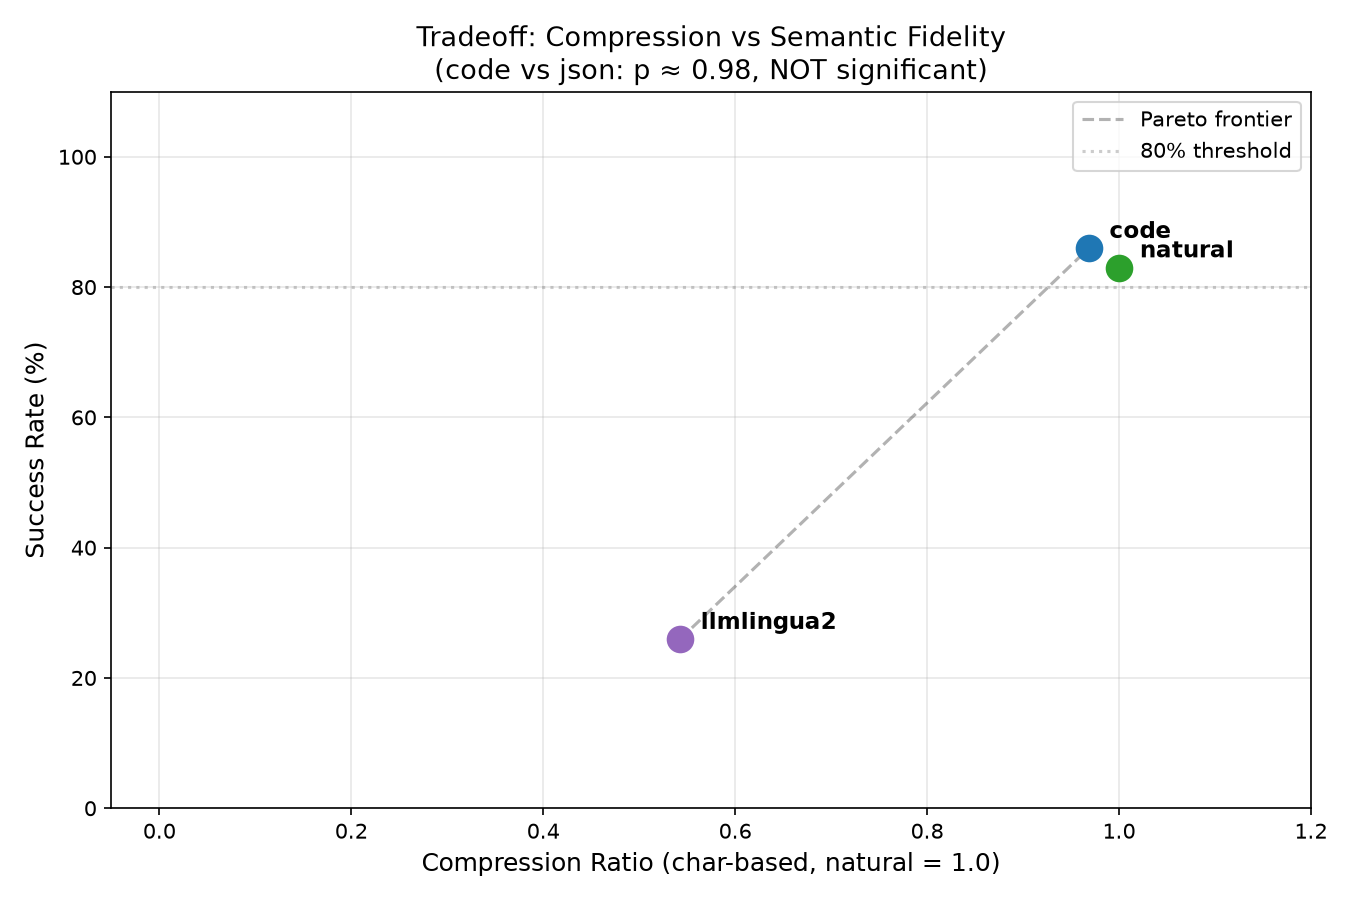
\includegraphics[width=0.9\textwidth]{tradeoff_curve}
\caption{Compression--accuracy tradeoff. The x-axis is compression ratio (1.0 = same length as natural language; \textless1.0 = shorter). The y-axis is pass rate. The code frontend occupies a favorable region: it achieves accuracy statistically indistinguishable from JSON (McNemar p = 0.855) at substantially lower character length than JSON (0.968 vs.~2.230) and slightly lower than natural language (0.968 vs.~1.000). LLMLingua-2 is in the ``compressed + inaccurate'' quadrant (lower-left). JSON is ``expanded + accurate'' (upper-right).}
\label{fig:fig6}
\end{figure}



\subsubsection{McNemar Pairwise Comparisons}\label{mcnemar-pairwise-comparisons}



\begin{table}[H]
\centering
\small
\caption{McNemar pairwise comparisons (n=135 paired observations per pair). $\chi^2$ computed with continuity correction $(|b-c|-1)^2/(b+c)$. Discordant pairs: b (A pass, B fail) and c (A fail, B pass). The three top frontends (code, JSON, natural) are pairwise indistinguishable. All comparisons involving NL+JSON or LLMLingua-2 are significant.}
\begin{tabular}{llllll}
\toprule
Pair & Rate A & Rate B & $\chi$$^{2}$ & p & Significant? \\
\midrule
Code vs.~JSON & 85.9\% & 84.4\% & 0.03 & 0.855 & No \\
Code vs.~Natural & 85.9\% & 83.0\% & 0.28 & 0.596 & No \\
Code vs.~NL+JSON & 85.9\% & 67.4\% & 11.29 & \textless0.001 & Yes \\
Code vs.~LLMLingua2 & 85.9\% & 25.9\% & 67.37 & \textless0.001 & Yes \\
JSON vs.~Natural & 84.4\% & 83.0\% & 0.03 & 0.860 & No \\
JSON vs.~NL+JSON & 84.4\% & 67.4\% & 10.30 & 0.001 & Yes \\
JSON vs.~LLMLingua2 & 84.4\% & 25.9\% & 66.86 & \textless0.001 & Yes \\
Natural vs.~NL+JSON & 83.0\% & 67.4\% & 8.51 & 0.004 & Yes \\
Natural vs.~LLMLingua2 & 83.0\% & 25.9\% & 62.11 & \textless0.001 & Yes \\
NL+JSON vs.~LLMLingua2 & 67.4\% & 25.9\% & 38.78 & \textless0.001 & Yes \\
\bottomrule
\end{tabular}
\end{table}


\subsubsection{Case-Level Analysis}\label{case-level-analysis}



\begin{figure}[H]
\centering

\includegraphics[width=0.9\textwidth]{fig5_case_level_grid}
\caption{Case $\times$ model pass/fail grid. Each cell is a binary pass (green) / fail (red) for one case under one frontend $\times$ model combination. The grid reveals that failures cluster on specific case types: negation logic (case 2 variants), conditional branching (case 7 variants), and multi-argument search (case 8 variants) are the most challenging across all frontends.}
\label{fig:fig5}
\end{figure}



\subsection{Phase 3: Ablation Study}\label{phase-3-ablation-study}



\subsubsection{Design}\label{design}



To probe sensitivity to syntactic order and semantic vocabulary, we transform each case's code-frontend compilation into three conditions:



\begin{enumerate}


\item

  \textbf{original}: The normal code-frontend output (e.g., \texttt{if\ !rain(t+1):\ start(hike)\ else\ start(cards@indoor)}).

\item

  \textbf{shuffled}: Word-level tokens of the original, randomly permuted. Destroys syntactic structure but preserves the exact vocabulary (e.g., \texttt{cards@indoor\ else\ start(t+1)\ if\ !rain(hike):\ start}).

\item

  \textbf{skeleton}: Syntactic skeleton preserved, all semantic identifiers replaced with meaningless tokens (e.g., \texttt{if\ !aaa(t+1):\ bbb(ccc)\ else\ bbb(ddd@eee)}).

\end{enumerate}



3 models (DeepSeek-v3.2, GLM-5.2, Kimi-K2.6) $\times$ 3 conditions $\times$ 27 cases = 243 runs.



\subsubsection{Results}\label{results-1}



\begin{table}[H]
\centering
\small
\caption{Ablation pass rates. The skeleton condition (syntax preserved, vocabulary removed) nearly completely collapses to 1.2\%, while the shuffled condition (vocabulary preserved, syntax destroyed) retains 55.6\%.}
\begin{tabular}{lllll}
\toprule
Condition & DeepSeek & GLM & Kimi & Overall \\
\midrule
Original & 22/27 (81.5\%) & 24/27 (88.9\%) & 24/27 (88.9\%) & 70/81 (\textbf{86.4\%}) \\
Shuffled & 12/27 (44.4\%) & 17/27 (63.0\%) & 16/27 (59.3\%) & 45/81 (\textbf{55.6\%}) \\
Skeleton & 1/27 (3.7\%) & 0/27 (0.0\%) & 0/27 (0.0\%) & 1/81 (\textbf{1.2\%}) \\
\bottomrule
\end{tabular}
\end{table}


\begin{figure}[ht]
\centering
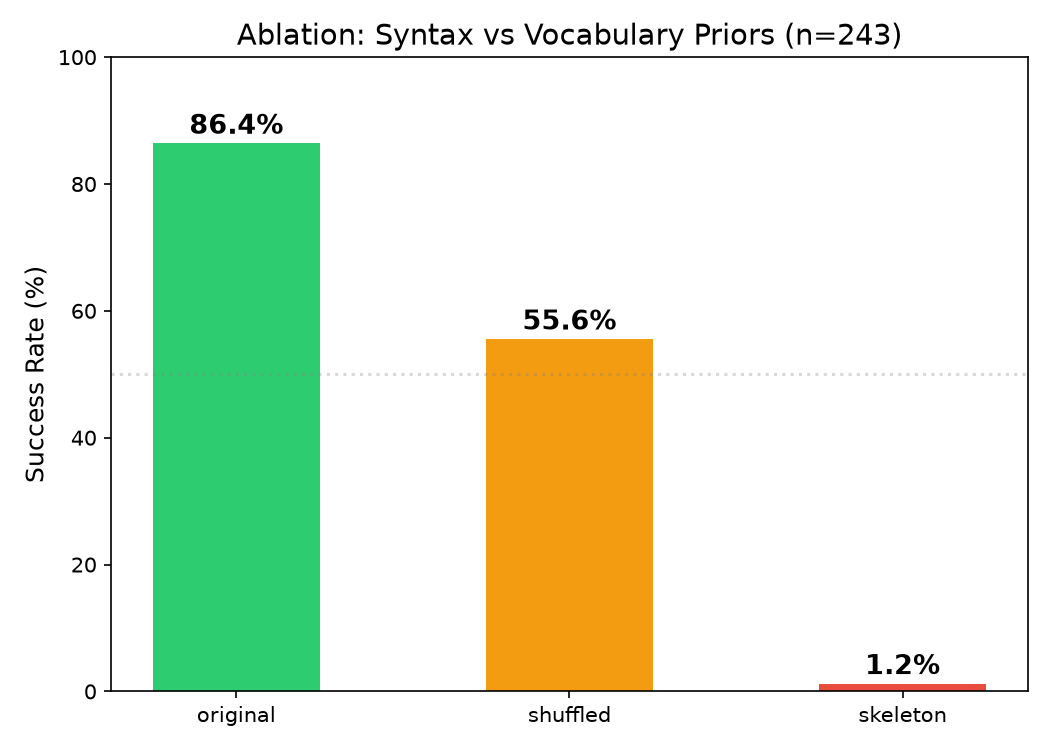
\includegraphics[width=0.9\textwidth]{ablation_overall}
\caption{Three-condition ablation pass rates. The original-to-skeleton drop measures sensitivity to semantic-vocabulary removal. The original-to-shuffled drop measures sensitivity to word-order disruption.}
\label{fig:fig7}
\end{figure}



\subsubsection{Perturbation Effects}\label{perturbation-effects}



\begin{itemize}



\item

  \textbf{Vocabulary perturbation effect} (original - skeleton = 86.4\% - 1.2\% = \textbf{85.2 pp}): Removing all vocabulary semantics while preserving syntax structure causes near-total collapse, indicating strong sensitivity to semantic-vocabulary removal.

\item

  \textbf{Syntax perturbation effect} (original - shuffled = 86.4\% - 55.6\% = \textbf{30.8 pp}): Preserving vocabulary but disrupting word order causes a 30.8 pp drop, indicating sensitivity to syntactic-order disruption.

\item

  \textbf{Descriptive ratio}: The vocabulary perturbation effect is 2.8$\times$ the syntax perturbation effect (85.2/30.8). Note: these are performance drops under two non-orthogonal perturbations, not independent causal contributions from a factorial design.

\end{itemize}



Statistical significance: McNemar's test confirms significant differences between original vs.~shuffled (p < 0.01) and original vs.~skeleton (p < 0.001).



\subsubsection{By-Category Breakdown}\label{by-category-breakdown}



\begin{figure}[H]
\centering
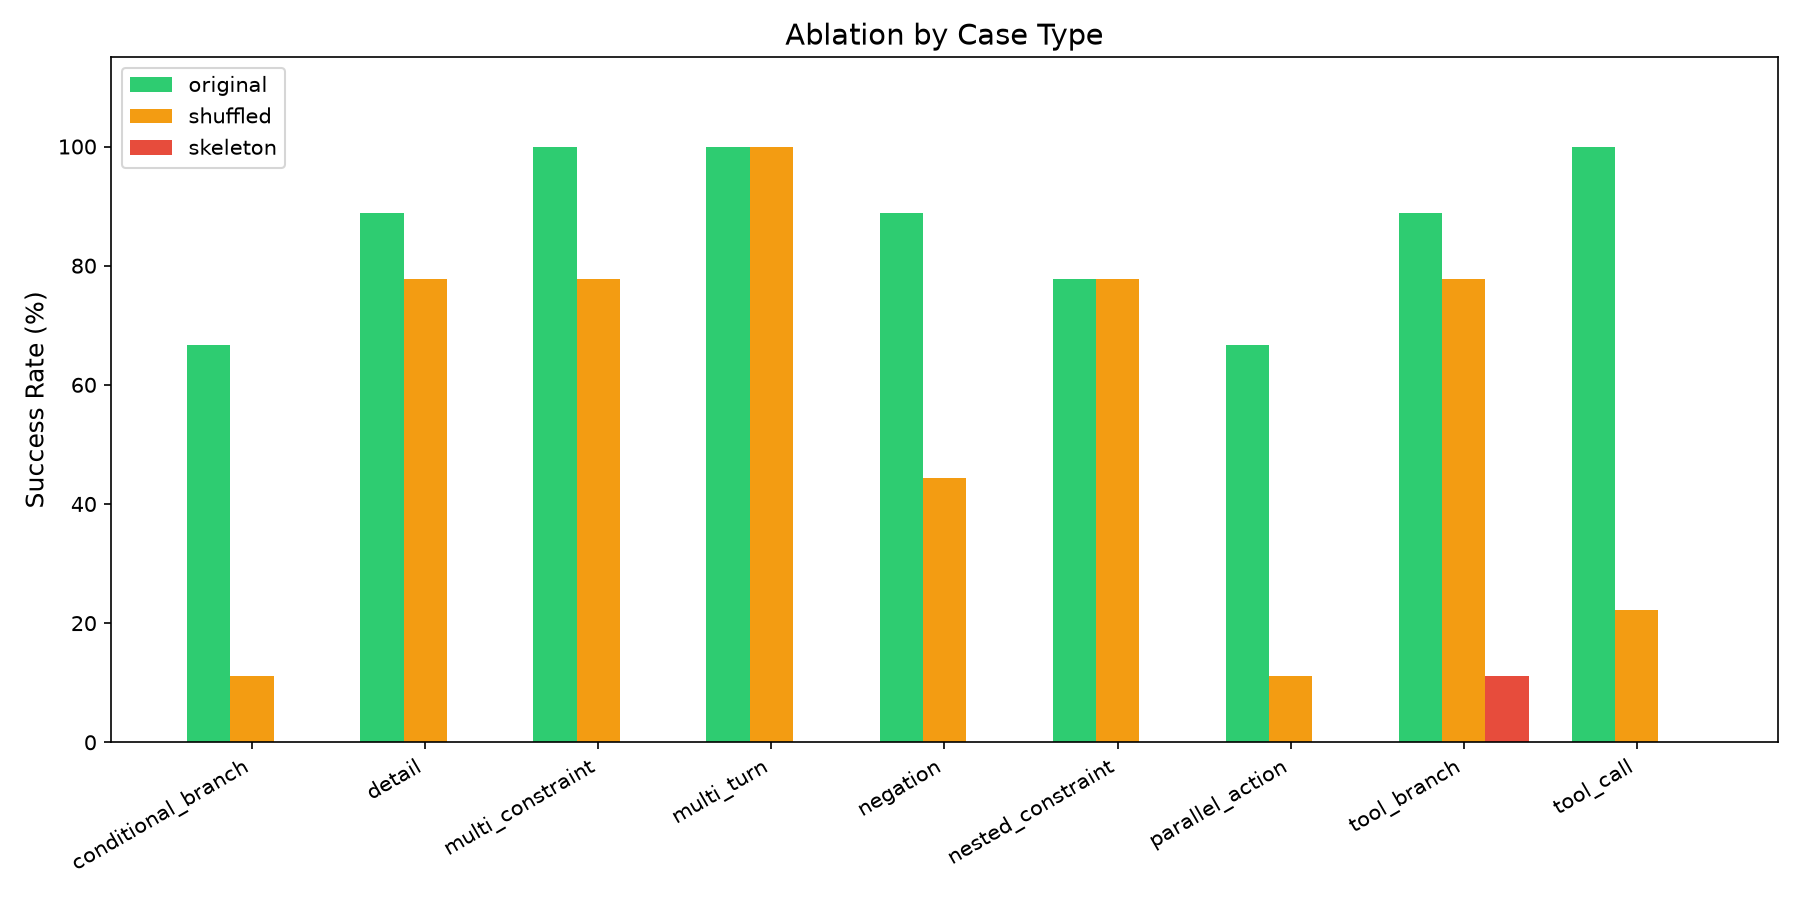
\includegraphics[width=0.9\textwidth]{ablation_by_type}
\caption{Ablation pass rates by case category. The skeleton condition (blue) is near-zero across all categories except \texttt{tool\_branch} (11\%). The shuffled condition (orange) shows high variance: \texttt{multi\_turn} and \texttt{detail} retain 100\% and 78\% respectively (likely because word reordering is less destructive for simple instructions), while \texttt{conditional\_branch} and \texttt{parallel\_action} collapse to 11\% (syntax order is critical for these categories).}
\label{fig:fig8}
\end{figure}



\begin{table}[H]
\centering
\small
\caption{Ablation by case category (n=9 per cell). The \texttt{conditional\_branch} and \texttt{parallel\_action} categories are most syntax-dependent (shuffled drops to 11\%), while \texttt{multi\_turn} is least affected by shuffling (100\%), likely because stateful update instructions are short and word-order-invariant.}
\begin{tabular}{llll}
\toprule
Category & Original & Shuffled & Skeleton \\
\midrule
Multi-constraint & 100\% & 78\% & 0\% \\
Negation & 89\% & 44\% & 0\% \\
Detail & 89\% & 78\% & 0\% \\
Tool branch & 89\% & 78\% & 11\% \\
Nested constraint & 78\% & 78\% & 0\% \\
Conditional branch & 67\% & 11\% & 0\% \\
Parallel action & 67\% & 11\% & 0\% \\
Tool call & 100\% & 22\% & 0\% \\
Multi-turn & 100\% & 100\% & 0\% \\
\bottomrule
\end{tabular}
\end{table}


\subsection{Phase 3: Entropy Analysis}\label{phase-3-entropy-analysis}



\subsubsection{Methodology}\label{methodology}



We initially attempted character-frequency entropy (monogram and bigram entropy) but found it biased toward JSON's frequent structural characters (\texttt{\{}, \texttt{\}}, \texttt{"}). We switched to \textbf{raw DEFLATE compression entropy} (bits/char), using \texttt{zlib.compress} with the raw DEFLATE window to strip header/trailer overhead, providing an estimate of empirical information density for short texts.



\subsubsection{Results}\label{results-2}



\begin{table}[H]
\centering
\small
\caption{DEFLATE entropy vs.~pass rate (n=135 per frontend). JSON has the lowest entropy (6.08 bits/char) due to highly repetitive structural tokens, while LLMLingua-2 has the highest (8.20) due to aggressive compression removing redundancy.}
\begin{tabular}{lll}
\toprule
Frontend & DEFLATE Entropy (bits/char) & Pass Rate \\
\midrule
LLMLingua2 & 8.20 & 25.9\% \\
Code & 7.55 & 85.9\% \\
Natural & 7.40 & 83.0\% \\
NL+JSON & 7.20 & 67.4\% \\
JSON & 6.08 & 84.4\% \\
\bottomrule
\end{tabular}
\end{table}


\begin{figure}[ht]
\centering

\includegraphics[width=0.9\textwidth]{entropy_curve}
\caption{DEFLATE entropy vs.~pass rate. No significant Spearman correlation was found (n=5, statistical power insufficient). The relationship is non-monotonic: JSON (low entropy, high pass rate) and LLMLingua-2 (high entropy, low pass rate) anchor opposite ends, but code and natural (similar entropy, similar pass rate) and NL+JSON (mid entropy, low pass rate) break any linear trend.}
\label{fig:fig9}
\end{figure}



\textbf{Statistical caveat}: With only n=5 frontends, the Spearman correlation between DEFLATE entropy and pass rate is not significant ($\rho$ = -0.30, p > 0.5, n=5). We explicitly note this as underpowered and do not draw causal conclusions from the entropy--accuracy relationship. The entropy data is reported descriptively only.



\subsection{Phase 3: Heartbeat N-Value Experiment}\label{phase-3-heartbeat-n-value-experiment}



\subsubsection{Design}\label{design-1}



We simulated stateful multi-turn sessions to test whether SILP-encoded instructions exhibit error propagation or pass-rate degradation over extended conversations:



\begin{itemize}



\item

  \textbf{6 N values}: 1 (stateless), 5, 10, 15, 20, 9999 (no heartbeat, stateful throughout)

\item

  \textbf{15 turns per session}, \textbf{8 random seeds} (different case orderings)

\item

  \textbf{3 models}: DeepSeek-v3.2, GLM-5.2, Kimi-K2.6

\item

  \textbf{Total}: 3 $\times$ 8 $\times$ 6 $\times$ 15 = \textbf{2,160 runs}

\end{itemize}



The N parameter controls heartbeat renewal frequency: in stateful mode, the session context accumulates over turns. N=1 is equivalent to stateless (context resets each turn), while N=9999 means the session never renews (maximum context accumulation).



\subsubsection{Error Propagation}\label{error-propagation}



We tested whether a failure on turn \emph{t} increases the probability of failure on turn \emph{t+1}:



\begin{table}[H]
\centering
\small
\caption{Error propagation analysis (Fisher exact test, two-sided). OR = odds ratio; CI = Woolf confidence interval. All three models' 95\% CIs cross 1.0, failing to reject the null hypothesis of no error propagation.}
\begin{tabular}{lllll}
\toprule
Model & P(fail\textbar prev pass) & P(fail\textbar prev fail) & OR (95\% CI) & p (two-sided) \\
\midrule
DeepSeek & 15.8\% & 23.0\% & 1.59 (0.93--2.71) & 0.105 \\
GLM & 9.7\% & 10.0\% & 1.04 (0.39--2.74) & 1.000 \\
Kimi & 9.0\% & 4.3\% & 0.46 (0.11--1.96) & 0.411 \\
\bottomrule
\end{tabular}
\end{table}


\begin{figure}[H]
\centering

\includegraphics[width=0.9\textwidth]{fig_heartbeat_error_propagation}
\caption{Error propagation comparison. For each model, the bar on the left shows P(fail \textbar{} previous turn passed) and the bar on the right shows P(fail \textbar{} previous turn failed). Error bars represent 95\% confidence intervals. The overlapping CIs indicate no significant error propagation effect.}
\label{fig:fig11}
\end{figure}



DeepSeek-v3.2 shows a \emph{point estimate} suggesting increased failure after a prior failure (23.0\% vs.~15.8\%, OR=1.59), but the 95\% CI (0.93--2.71) is wide and crosses 1.0, precluding any conclusion. GLM-5.2 and Kimi-K2.6 show ORs near or below 1.0 (1.04 and 0.46 respectively), with CIs broadly spanning 1.0.



\subsubsection{Context Depth Trends}\label{context-depth-trends}



We tested whether pass rate or latency changes with context depth (number of preceding turns in the session):



\begin{table}[H]
\centering
\small
\caption{Spearman's $\rho$ between pass rate/latency and context depth (n=15 distinct context-depth levels, 0--14). No pass-rate trend is significant (all p > 0.2). Latency trends are significant for DeepSeek ($\rho$=+0.900, p = 0.000005) and GLM ($\rho$=+0.829, p = 0.000135), confirming expected context-length-induced latency increase. Kimi shows no significant latency trend ($\rho$=+0.375, p = 0.168).}
\begin{tabular}{lllll}
\toprule
Model & Pass Rate $\rho$ & p & Latency $\rho$ & p \\
\midrule
DeepSeek & +0.099 & 0.726 & +0.900 & 0.000005 \\
GLM & +0.327 & 0.234 & +0.829 & 0.000135 \\
Kimi & +0.195 & 0.486 & +0.375 & 0.168 \\
\bottomrule
\end{tabular}
\end{table}


\begin{figure}[H]
\centering

\includegraphics[width=0.9\textwidth]{fig_heartbeat_passrate_by_context}
\caption{Pass rate vs.~context depth. No systematic degradation pattern was detected across context depths 0--14 for all three models.}
\label{fig:fig10}
\end{figure}



\begin{figure}[H]
\centering

\includegraphics[width=0.9\textwidth]{fig_heartbeat_latency}
\caption{Latency vs.~context depth. DeepSeek and GLM show steep latency increases ($\rho$ $\geq$ 0.83, p < 0.001), while Kimi's trend is non-significant.}
\label{fig:fig14}
\end{figure}



\subsubsection{N-Value Overall Pass Rates}\label{n-value-overall-pass-rates}



\begin{table}[H]
\centering
\small
\caption{Pass rates by N value (n=120 per cell, 8 seeds $\times$ 15 turns). No systematic pattern of degradation with increasing N is observed. GLM and Kimi remain stable at 86--93\% across all N values. DeepSeek shows non-monotonic variation (76.7--87.5\%) but no downward trend.}
\begin{tabular}{lllllll}
\toprule
Model & N=1 & N=5 & N=10 & N=15 & N=20 & N=9999 \\
\midrule
DeepSeek & 76.7\% & 81.7\% & 80.0\% & 85.0\% & 87.5\% & 77.5\% \\
GLM & 90.8\% & 86.7\% & 87.5\% & 90.8\% & 91.7\% & 92.5\% \\
Kimi & 90.0\% & 92.5\% & 90.8\% & 92.5\% & 89.2\% & 92.5\% \\
\bottomrule
\end{tabular}
\end{table}


\begin{figure}[H]
\centering

\includegraphics[width=0.9\textwidth]{fig_heartbeat_n_overall}
\caption{Overall pass rates by N value. No monotonic relationship between heartbeat interval N and pass rate was observed.}
\label{fig:fig12}
\end{figure}



\begin{figure}[H]
\centering

\includegraphics[width=0.9\textwidth]{fig_heartbeat_turn_heatmap}
\caption{N $\times$ turn pass-rate heatmap. The heatmap shows no systematic ``darkening'' (failure clustering) in later turns.}
\label{fig:fig13}
\end{figure}



\subsubsection{Multiple Comparison Correction}\label{multiple-comparison-correction}



The heartbeat experiment involved 12 hypothesis tests (3 models $\times$ 4 tests: error propagation, pass-rate trend, N=1 vs.~N=$\infty$, latency trend). Across the full project, 35 tests were conducted (10 Phase 2 cross-model Spearman correlations in \S4.4.2, 10 Phase 2 pairwise McNemar comparisons in Table 7, 2 Phase 3 ablation McNemar tests in \S4.5.3, 12 heartbeat tests, and 1 entropy--accuracy Spearman in \S4.6; see Appendix B). Applying Benjamini--Hochberg FDR correction across all 35 tests:



\begin{itemize}



\item

  \textbf{20 tests survive} at q < 0.05: 9 of 10 Phase 2 cross-model Spearman tests (the non-surviving test is DeepSeek vs.~Kimi, p = 0.034, q = 0.056), 7 of 10 Phase 2 McNemar comparisons (the three non-surviving comparisons are code vs.~json, code vs.~natural, and json vs.~natural---all pairwise among the top three frontends), both ablation McNemar tests, and 2 heartbeat latency-trend tests.

\item

  \textbf{Among the 12 heartbeat tests}, only the two latency trends (DeepSeek $\rho$=+0.900, GLM $\rho$=+0.829) survive. The 9 accuracy-related heartbeat tests (error propagation, pass-rate trends, N=1 vs.~N=$\infty$) remain non-significant after correction.

\end{itemize}



\textbf{Conclusion}: We found no statistically significant evidence of pass-rate degradation or error propagation within the tested 15-turn setting. This should not be interpreted as evidence of equivalence or absence of small effects, particularly given the underpowering at deep context depths.



\subsubsection{Experimental Design Limitations}\label{experimental-design-limitations}



We note two structural limitations:



\begin{enumerate}


\item

  \textbf{N=15/20/9999 structural equivalence}: In a 15-turn session, the heartbeat never triggers for N $\geq$ 15 (since the session ends before renewal is needed). Thus N=15, N=20, and N=9999 are behaviorally identical.

\item

  \textbf{Deep context underpowering}: Context depth 10--14 has only 24 observations per cell (from 8 seeds $\times$ 3 late turns), limiting statistical power to detect trends at \textbar $\rho$\textbar{} < 0.52. Context depth 0 has 184--185 observations (every session's first turn).

\end{enumerate}



\section{Discussion}\label{discussion}



\subsection{Falsifying the Central Hypothesis}\label{falsifying-the-central-hypothesis}



The original hypothesis predicted that ``shared syntax priors > shared vocabulary priors.'' The ablation results (\S4.5) contradict this directional prediction: \emph{both} perturbations produce significant effects, but removing semantic vocabulary causes a 2.8$\times$ larger performance drop than shuffling syntactic order (85.2 pp vs.~30.8 pp). This is not a refinement but a reversal of the predicted ordering. The code frontend's overall advantage over natural language (85.9\% vs.~83.0\%, not significant) cannot be attributed solely to syntax format---the larger performance drop under vocabulary removal suggests stronger sensitivity to semantic vocabulary than to the tested syntactic perturbation.



\subsection{The NL+JSON Surprise}\label{the-nljson-surprise}



The most unexpected finding is that wrapping natural language in a JSON container \emph{degrades} comprehension by 15.6 pp (83.0\% $\to$ 67.4\%, p = 0.004). This contradicts the intuitive expectation that structured containers help models parse content. We hypothesize that the wrapper introduces additional structural tokens and key names that may dilute the semantic signal or alter how models interpret the payload, and that models may attempt to ``parse'' the JSON structure rather than reading the prose---introducing a parsing failure mode that doesn't exist in bare natural language. This finding has practical implications for agent protocol design: wrapping unstructured content in JSON does not help and may hurt.



\subsection{Compression vs.~Protocol}\label{compression-vs.-protocol}



The 60 pp gap between LLMLingua-2 (25.9\%) and code (85.9\%) under the tested configuration (rate=0.5) is the most practically significant finding. It shows that this particular ML-based prompt compression setting, while effective at reducing character length, substantially reduces the semantic precision necessary for inter-agent communication. Error inspection suggests that the tested compression configuration may remove or obscure negation markers and entity boundaries, particularly in cases involving negation logic. SILP's structured frontends achieve compression \emph{and} accuracy by \emph{designing} the encoding to be both compact and semantically complete, rather than \emph{compressing} an existing encoding post-hoc.



\subsection{Cross-Model Consistency}\label{cross-model-consistency}



The Spearman analysis (\S4.4.2) shows weak-to-moderate agreement across all model pairs ($\rho$=0.18--0.54, 9 of 10 significant after BH-FDR). This means that models tend to agree on which case--frontend combinations are easy or difficult. It also provides preliminary motivation for the migration screening layer's premise (Layer 5): if models agree on relative difficulty, small models may serve as screening proxies for frontend evaluation, though this has not been directly validated.



\subsection{Multi-Turn Robustness}\label{multi-turn-robustness}



The heartbeat experiment found no statistically significant evidence of error propagation or pass-rate degradation across 15 turns. However, we caution that 15 turns may not capture truly long conversations (100+ turns), and the structural equivalence of N=15/20/9999 limits the N-value comparison's power.



\section{Limitations}\label{limitations}



\begin{enumerate}


\item

  \textbf{Sample size for entropy analysis}: The entropy--accuracy relationship (\S4.6) is based on only n=5 frontends, yielding insufficient statistical power. We explicitly retract any causal claim from this analysis and report it descriptively only.

\item

  \textbf{Deep context underpowering}: In the heartbeat experiment, context depths 10--14 have only 24 observations per cell. While no trend was detected, the power to detect small effects (\textbar $\rho$\textbar{} < 0.52) is limited.

\item

  \textbf{N-value structural equivalence}: N=15, 20, and 9999 are behaviorally identical in 15-turn sessions. The N-value comparison effectively has only 3 distinct conditions (N=1, 5, 10) rather than 6.

\item

  \textbf{No human readability evaluation}: The protocol spec defines a human-readability gradient (PPL, decode time, semantic reconstruction, learning-then-retest, by technical/non-technical population), but this experiment has not yet been conducted. We cannot make claims about human interpretability of SILP encodings.

\item

  \textbf{Single judge model}: The LLM judge uses GLM-5.2 exclusively. Judge bias---particularly systematic over/under-scoring of models from the same family---is possible. The rule judge provides a limited cross-check but cannot detect semantic false positives.

\item

  \textbf{Model identity not verified}: All five models were accessed through a single OpenAI-compatible proxy. We cannot independently verify that API requests were routed to the claimed model endpoints. If the proxy misrouted requests (e.g., serving a different model for one provider), the cross-model comparison matrix would be compromised.

\item

  \textbf{27 test cases}: While the 27 cases span 9 semantic categories with 3 difficulty variants, they may not represent the full diversity of agent-to-agent communication tasks (e.g., multi-modal, long-horizon planning, negotiation).

\item

  \textbf{Partial protocol implementation}: Of the five SILP layers, Layer 1 (IR) and Layer 2 (frontends) are fully experimentally validated. Layer 3 (meta-protocol) is partially tested---the heartbeat experiment tests session management and error propagation, but \texttt{//ping} negotiation probes and degradation chains are design-only. Layer 5 (migration) remains unvalidated---the production-model agreement analysis (\S4.4.2) provides only preliminary motivation and does not test small-model screening or frontend-rank preservation directly. Layer 4 (optimization) is design-only---the fitness function is defined but never evaluated.

\item

  \textbf{No Phase 4 experiments}: The optimization layer (Layer 4), migration screening layer (Layer 5), cross-language experiments, and automatic evolution have not been implemented or evaluated. These are planned for Phase 4.

\end{enumerate}



\section{Future Work}\label{future-work}



\subsection{Phase 4: Automatic Evolution and Negotiation}\label{phase-4-automatic-evolution-and-negotiation}



Implement and evaluate the optimization layer (Layer 4) with the multi-objective fitness function, using genetic algorithms for semantic-level crossover of IR structures. The migration screening layer (Layer 5) will be validated by training small proxy models (SmolLM-360M, Qwen2.5-0.5B) and measuring Spearman ranking preservation against API-reported endpoints.



\subsection{Cross-Language Experiments}\label{cross-language-experiments}



Test the hypothesis that English-verb frontends (\texttt{cancel(flight)}) and pure-symbol action-code frontends (\texttt{!CANCEL}) perform differently across models trained on different language distributions. This includes an ``English verb vs.~pure symbol action code'' controlled comparison.



\subsection{Human Readability Evaluation}\label{human-readability-evaluation}



Conduct the planned human-readability study: 10 technical + 10 non-technical participants, decode-time measurement, semantic reconstruction task, and learning-then-retest calibration. This will determine whether SILP encodings are human-auditable in practice, not just in principle.



\subsection{Longer Multi-Turn Sessions}\label{longer-multi-turn-sessions}



Extend the heartbeat experiment to 100+ turns with larger N values to test whether error propagation eventually emerges in truly long conversations. The current 15-turn design is limited by API cost and proxy reliability.



\subsection{Judge Sensitivity Analysis}\label{judge-sensitivity-analysis}



Evaluate multiple LLM judges (e.g., GPT-4o, Claude-3.5, DeepSeek-v3.2) to measure judge bias and establish inter-judge agreement rates. This would address the single-judge limitation.



\subsection{Dynamic Negotiation Evaluation}\label{dynamic-negotiation-evaluation}



Implement and test the \texttt{//ping} probe-based negotiation protocol: measure the token cost of negotiation vs.~default-frontend selection, and determine the breakeven point where negotiation becomes worthwhile.



\section{Conclusion}\label{conclusion}



We presented SILP, a five-layer protocol for encoding semantic payloads in LLM agent communication. Through a systematic experimental program across four main phases plus a smoke-test subphase (3,159 total model invocations), we demonstrated that: (1) code-like function-call syntax achieves the highest average pass rate (85.9\%, statistically tied with JSON and natural language) with the lowest tokenizer variance; (2) both perturbations produced significant effects, with vocabulary removal causing a 2.8$\times$ larger performance drop than word-order shuffling (85.2 vs.~30.8 pp); (3) under the tested LLMLingua-2 configuration (rate=0.5), the code frontend exceeds the tested LLMLingua-2 baseline by 60.0 pp; and (4) we detected no statistically significant evidence of error propagation or pass-rate degradation within 15-turn sessions, though the experiment is underpowered for small deep-context effects. The implemented codec, benchmark harness, protocol specification, and raw data are released as open-source at https://github.com/Juwan-Hwang/polyglotir to support reproducibility and further research.



\appendix\section{Appendix A: Figure Index}\label{appendix-a-figure-index}



\begin{table}[ht]
\centering
\footnotesize
\caption{Figure index.}
\begin{tabular}{p{1.2cm}p{7.5cm}p{4cm}}
\toprule
Figure & Filename & Description \\
\midrule
Figure 1 & \texttt{fig3\_token\_variance} & Phase 0 tokenizer variance \\
Figure 2 & \texttt{fig1\_passrate\_heatmap} & Phase 2 pass-rate heatmap \\
Figure 3 & \texttt{fig4\_frontend\_ranking} & Phase 2 frontend ranking \\
Figure 4 & \texttt{fig2\_spearman\_bar} & Cross-model Spearman correlations \\
Figure 5 & \texttt{tradeoff\_curve} & Compression--accuracy tradeoff \\
Figure 6 & \texttt{fig5\_case\_level\_grid} & Case-level pass/fail grid \\
Figure 7 & \texttt{ablation\_overall} & Overall ablation results \\
Figure 8 & \texttt{ablation\_by\_type} & Ablation by category \\
Figure 9 & \texttt{entropy\_curve} & Entropy--accuracy analysis \\
Figure 10 & \texttt{fig\_heartbeat\_error\_propagation} & Error propagation \\
Figure 11 & \texttt{fig\_heartbeat\_passrate\_by\_context} & Pass rate vs.~context depth \\
Figure 12 & \texttt{fig\_heartbeat\_latency} & Latency vs.~context depth \\
Figure 13 & \texttt{fig\_heartbeat\_n\_overall} & Overall pass rate by heartbeat $N$ \\
Figure 14 & \texttt{fig\_heartbeat\_turn\_heatmap} & $N$ $\times$ turn heatmap \\
\bottomrule
\end{tabular}
\end{table}


\section{Appendix B: Complete List of Hypothesis Tests}\label{appendix-b-complete-list-of-hypothesis-tests}



All 35 hypothesis tests, sorted by raw p-value with Benjamini--Hochberg FDR correction (m=35, significance threshold q\textless0.05). McNemar $\chi$$^{2}$ uses continuity correction \texttt{(\textbar{}b-c\textbar{}-1)$^{2}$/(b+c)}; b and c are discordant pair counts. P-values were computed using the specified SciPy procedures and reported at full numerical precision. Fisher's exact test is exact; McNemar comparisons use the asymptotic chi-square approximation with continuity correction. Specific procedures: \texttt{scipy.stats.chi2.sf} (McNemar), \texttt{scipy.stats.fisher\_exact} (Fisher), \texttt{scipy.stats.spearmanr} (Spearman), \texttt{scipy.stats.chi2\_contingency} (N=1 vs N=$\infty$).



\begin{table}[ht]
\centering
\scriptsize
\caption{All 35 hypothesis tests with BH-FDR correction.}
\begin{tabular}{p{0.4cm}p{3.5cm}p{2.8cm}p{1.0cm}p{1.0cm}p{0.6cm}}
\toprule
Rank & Test & Statistic & Raw p & BH q & Decision \\
\midrule
1 & McNemar: code vs llmlingua2 & $\chi$$^{2}$=67.37, b=88, c=7 & 2.25$\times$10$^{-}$$^{1}$$^{6}$ & 3.41$\times$10$^{-}$$^{1}$$^{5}$ & Reject \\
2 & McNemar: original vs skeleton & b=69, c=0, $\chi$$^{2}$=67.01 & 2.70$\times$10$^{-}$$^{1}$$^{6}$ & 3.41$\times$10$^{-}$$^{1}$$^{5}$ & Reject \\
3 & McNemar: json vs llmlingua2 & $\chi$$^{2}$=66.86, b=85, c=6 & 2.92$\times$10$^{-}$$^{1}$$^{6}$ & 3.41$\times$10$^{-}$$^{1}$$^{5}$ & Reject \\
4 & McNemar: natural vs llmlingua2 & $\chi$$^{2}$=62.11, b=85, c=8 & 3.25$\times$10$^{-}$$^{1}$$^{5}$ & 2.85$\times$10$^{-}$$^{1}$$^{4}$ & Reject \\
5 & Spearman: GLM vs LongCat & $\rho$=0.538 & 1.78$\times$10$^{-}$$^{1}$$^{1}$ & 1.25$\times$10$^{-}$$^{1}$$^{0}$ & Reject \\
6 & McNemar: nl\_json vs llmlingua2 & $\chi$$^{2}$=38.78, b=67, c=11 & 4.74$\times$10$^{-}$$^{1}$$^{0}$ & 2.76$\times$10$^{-}$$^{9}$ & Reject \\
7 & Spearman: LongCat vs MiniMax & $\rho$=0.469 & 9.42$\times$10$^{-}$$^{9}$ & 4.71$\times$10$^{-}$$^{8}$ & Reject \\
8 & Spearman: DeepSeek vs LongCat & $\rho$=0.439 & 9.94$\times$10$^{-}$$^{8}$ & 4.35$\times$10$^{-}$$^{7}$ & Reject \\
9 & Spearman: GLM vs MiniMax & $\rho$=0.432 & 1.64$\times$10$^{-}$$^{7}$ & 6.39$\times$10$^{-}$$^{7}$ & Reject \\
10 & Spearman: DeepSeek vs GLM & $\rho$=0.411 & 7.55$\times$10$^{-}$$^{7}$ & 2.64$\times$10$^{-}$$^{6}$ & Reject \\
11 & Spearman: DS latency vs context & $\rho$=+0.900 & 4.87$\times$10$^{-}$$^{6}$ & 1.55$\times$10$^{-}$$^{5}$ & Reject \\
12 & Spearman: Kimi vs MiniMax & $\rho$=0.353 & 2.74$\times$10$^{-}$$^{5}$ & 8.00$\times$10$^{-}$$^{5}$ & Reject \\
13 & Spearman: GLM vs Kimi & $\rho$=0.344 & 4.30$\times$10$^{-}$$^{5}$ & 1.16$\times$10$^{-}$$^{4}$ & Reject \\
14 & McNemar: original vs shuffled & b=30, c=5, $\chi$$^{2}$=16.46 & 4.98$\times$10$^{-}$$^{5}$ & 1.24$\times$10$^{-}$$^{4}$ & Reject \\
15 & Spearman: GLM latency vs context & $\rho$=+0.829 & 1.35$\times$10$^{-}$$^{4}$ & 3.16$\times$10$^{-}$$^{4}$ & Reject \\
16 & Spearman: DeepSeek vs MiniMax & $\rho$=0.309 & 2.65$\times$10$^{-}$$^{4}$ & 5.80$\times$10$^{-}$$^{4}$ & Reject \\
17 & Spearman: Kimi vs LongCat & $\rho$=0.307 & 2.94$\times$10$^{-}$$^{4}$ & 6.06$\times$10$^{-}$$^{4}$ & Reject \\
18 & McNemar: code vs nl\_json & $\chi$$^{2}$=11.29, b=38, c=13 & 7.78$\times$10$^{-}$$^{4}$ & 1.51$\times$10$^{-}$$^{3}$ & Reject \\
19 & McNemar: json vs nl\_json & $\chi$$^{2}$=10.30, b=35, c=12 & 1.33$\times$10$^{-}$$^{3}$ & 2.45$\times$10$^{-}$$^{3}$ & Reject \\
20 & McNemar: natural vs nl\_json & $\chi$$^{2}$=8.51, b=34, c=13 & 3.53$\times$10$^{-}$$^{3}$ & 6.18$\times$10$^{-}$$^{3}$ & Reject \\
21 & Spearman: DeepSeek vs Kimi & $\rho$=0.183 & 3.35$\times$10$^{-}$$^{2}$ & 5.59$\times$10$^{-}$$^{2}$ & Retain \\
22 & Fisher: DS error propagation & OR, table={[}{[}367,69{]},{[}77,23{]}{]} & 1.05$\times$10$^{-}$$^{1}$ & 1.67$\times$10$^{-}$$^{1}$ & Retain \\
23 & Spearman: Kimi latency vs context & $\rho$=+0.375 & 1.68$\times$10$^{-}$$^{1}$ & 2.56$\times$10$^{-}$$^{1}$ & Retain \\
24 & Spearman: GLM pass-rate vs context & $\rho$=+0.327 & 2.34$\times$10$^{-}$$^{1}$ & 3.41$\times$10$^{-}$$^{1}$ & Retain \\
25 & Fisher: Kimi error propagation & OR, table={[}{[}445,44{]},{[}44,2{]}{]} & 4.11$\times$10$^{-}$$^{1}$ & 5.75$\times$10$^{-}$$^{1}$ & Retain \\
26 & Spearman: Kimi pass-rate vs context & $\rho$=+0.195 & 4.86$\times$10$^{-}$$^{1}$ & 6.54$\times$10$^{-}$$^{1}$ & Retain \\
27 & McNemar: code vs natural & $\chi$$^{2}$=0.28, b=18, c=14 & 5.96$\times$10$^{-}$$^{1}$ & 7.72$\times$10$^{-}$$^{1}$ & Retain \\
28 & Spearman: entropy vs pass rate & $\rho$=-0.300 & 6.24$\times$10$^{-}$$^{1}$ & 7.80$\times$10$^{-}$$^{1}$ & Retain \\
29 & N=1 vs N=$\infty$: Kimi ($\chi$$^{2}$) & $\chi$$^{2}$=0.21 & 6.48$\times$10$^{-}$$^{1}$ & 7.82$\times$10$^{-}$$^{1}$ & Retain \\
30 & Spearman: DS pass-rate vs context & $\rho$=+0.099 & 7.26$\times$10$^{-}$$^{1}$ & 8.47$\times$10$^{-}$$^{1}$ & Retain \\
31 & N=1 vs N=$\infty$: GLM ($\chi$$^{2}$) & $\chi$$^{2}$=0.05 & 8.15$\times$10$^{-}$$^{1}$ & 9.12$\times$10$^{-}$$^{1}$ & Retain \\
32 & McNemar: code vs json & $\chi$$^{2}$=0.03, b=16, c=14 & 8.55$\times$10$^{-}$$^{1}$ & 9.12$\times$10$^{-}$$^{1}$ & Retain \\
33 & McNemar: json vs natural & $\chi$$^{2}$=0.03, b=17, c=15 & 8.60$\times$10$^{-}$$^{1}$ & 9.12$\times$10$^{-}$$^{1}$ & Retain \\
34 & N=1 vs N=$\infty$: DeepSeek ($\chi$$^{2}$) & $\chi$$^{2}$=0.00 & 1.00$\times$10$^{0}$ & 1.00$\times$10$^{0}$ & Retain \\
35 & Fisher: GLM error propagation & OR, table={[}{[}439,47{]},{[}45,5{]}{]} & 1.00$\times$10$^{0}$ & 1.00$\times$10$^{0}$ & Retain \\
\bottomrule
\end{tabular}
\end{table}


\textbf{Summary}: 20 of 35 tests reject the null at q < 0.05. The 15 retained tests include all 9 heartbeat accuracy tests (error propagation, pass-rate trends, N=1 vs.~N=$\infty$), the 3 pairwise comparisons among the top three frontends (code vs.~json, code vs.~natural, json vs.~natural), the DeepSeek vs.~Kimi cross-model correlation, Kimi's latency trend, and the entropy--accuracy correlation.



\section{Appendix C: Table Index}\label{appendix-c-table-index}



\begin{table}[ht]
\centering
\small
\caption{Table index.}
\begin{tabular}{p{1.2cm}p{0.8cm}p{5cm}}
\toprule
Table & Section & Description \\
\midrule
Table 1 & \S3.1 & Five surface frontends \\
Table 2 & \S3.2 & Nine semantic categories (27 cases) \\
Table 3 & \S4.2 & Phase 0.5 smoke test pass rates \\
Table 4 & \S4.3 & req\_id collision test \\
Table 5 & \S4.4 & Phase 2 pass-rate matrix \\
Table 6 & \S4.4 & Compression--accuracy tradeoff \\
Table 7 & \S4.4 & McNemar pairwise comparisons \\
Table 8 & \S4.5 & Ablation pass rates \\
Table 9 & \S4.5 & Ablation by case category \\
Table 10 & \S4.6 & DEFLATE entropy vs.~pass rate \\
Table 11 & \S4.7 & Error propagation (Fisher exact) \\
Table 12 & \S4.7 & Context depth trends (Spearman $\rho$) \\
Table 13 & \S4.7 & N-value overall pass rates \\
\bottomrule
\end{tabular}
\end{table}



\clearpage
\small
\bibliographystyle{unsrtnat}
\bibliography{references}

\end{document}
